\section{Динамика}

%1
\AddProb На наклонной поверхности с углом $\alpha$ горизонту находится брусок. 
Коэффициент трения бруска о поверхность равен $\mu$. С каким ускорением будет двигаться брусок?

\begin{wrapfigure}{r}{5cm}
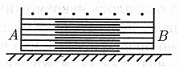
\includegraphics{0402DynamicsPaper.jpg}
\end{wrapfigure}

\AddProb Листы бумаги, сложенные, как показано на рисунке, склеивают свободными концами через лист таким образом, 
что получаются две самостоятельные кипы $A$ и $B$. Вес каждого листа 0.06 Н, число всех листов 200, коэффициент трения бумаги о бумагу, 
а также о стол, на котором бумага лежит, равен 0.2. Предполагая, что одна из кип удерживается неподвижно, 
определить наименьшее горизонтальное усилие $F$, необходимое для того, чтобы вытащить вторую кипу.

\begin{wrapfigure}{r}{3cm}
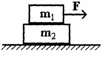
\includegraphics{0403DynamicsBlocks.jpg}
\end{wrapfigure}

\AddProb При какой максимальной силе $F$ верхний брусок еще не будет скользить по нижнему? 
Массы брусков $m_1$ и $m_2$, коэффициент трения между ними $\mu$, поверхность стола гладкая.

\AddProb По наклонной плоскости, образующей угол $\alpha$ с горизонтом, за веревку вытягивают ящик массы $M$. 
Коэффициент трения ящика о плоскость равен $\mu$. Под каким углом $\beta$ к горизонту следует тянуть веревку, 
чтобы равномерно двигать ящик с наименьшим усилием? Каково это усилие?

\begin{wrapfigure}{r}{2.5cm}
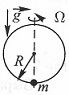
\includegraphics{0405DynamicsRing.jpg}
\end{wrapfigure}

\AddProb По вертикально подвешенному в поле тяжести Земли кольцу радиуса $R$ может скользить без трения шарик массы $m$. 
В начальный момент времени кольцо неподвижно, и шарик находится в нижней точке кольца. 
Как будет двигаться шарик, если кольцо начнет вращаться вокруг вертикальной оси с угловой скоростью $\omega$?

\begin{wrapfigure}{r}{3.5cm}
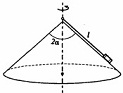
\includegraphics{0406DynamicsCone.jpg}
\end{wrapfigure}

%6
\AddProb К вершине прямого кругового конуса с помощью нити длиной $L$ прикреплена небольшая шайба. 
Вся система вращается вокруг оси конуса, расположенной вертикально. 
При каком числе оборотов в единицу времени шайба не будет отрываться от поверхности конуса? Угол при вершине конуса $2\alpha$.

\AddProb У края диска радиусом $R$ лежит монета. Диск раскручивается так, 
что его угловая скорость линейно растет со временем по закону $\omega = \varepsilon t$. 
В какой момент времени монета слетит с диска, если коэффициент трения между диском и монетой равен $\mu$? 
Какой угол с направлением к центру диска образует сила трения в этот момент?

\AddProb Найдите ускорения призмы массой $m_1$ и куба массой $m_2$, изображенных на рисунке. Трением пренебречь.

\begin{figure}[!h]
	\begin{subfigure}{.5\textwidth}
		\centering
		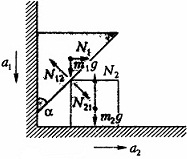
\includegraphics{0408DynamicsPrismAndCube.jpg}
	\end{subfigure}
	\begin{subfigure}{.5\textwidth}
		\centering
		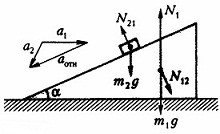
\includegraphics{0409DynamicsWedge.jpg}
	\end{subfigure}
\end{figure}

\AddProb Клин высотой $h$ с углом наклона $\alpha$ стоит на гладкой горизонтальной поверхности. 
Масса клина $m_1$. С вершины клина начинает соскальзывать без трения брусок массой $m_2$. Найдите ускорение клина и время соскальзывания бруска.

\begin{wrapfigure}{r}{2.5cm}
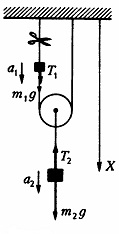
\includegraphics{0410DynamicsPulley.jpg}
\end{wrapfigure}

\AddProb Найдите ускорения грузов массой $m_1$ и $m_2$ после перерезания нити. Нить и блок считать идеальными.
